\documentclass[11pt]{article}

%use European style
\usepackage[a4paper,left=2cm,right=2cm,top=2cm,bottom=2cm]{geometry}

%few useful packages ------------------------------------------------------------------
	\usepackage{setspace}
		\let\Tiny=\tiny %remove annoying warnings
	\usepackage[english]{babel}
	\usepackage[latin1]{inputenc}
	\usepackage{amsfonts}
	\usepackage{amsmath}
	\usepackage{amssymb}
	\usepackage{amsthm}
	\usepackage{amsfonts}
	\usepackage{colortbl}
	\usepackage{float}
	\usepackage{xcolor}
	\usepackage{eurosym}
	\usepackage{enumitem}
	\usepackage{chngpage}
	\usepackage{fancyhdr}
	\usepackage{fancyvrb}
	\usepackage{float}
	\usepackage{framed}
	\usepackage{multirow}
	\usepackage{physics}
	\usepackage{graphicx}
		\graphicspath{ {./images/} }
	\usepackage{geometry}
	\usepackage{lipsum}
	\usepackage{tabularx}
	\usepackage{url}
	\usepackage[linktocpage]{hyperref}
	
	%define environment for code
	\definecolor{orangepse}{RGB}{240,139,39}
	\definecolor{redpse}{RGB}{222,6,61}
	\newcommand{\rpse}[1]{\textcolor{redpse}{#1}}
	\definecolor{dkgreen}{rgb}{0,0.6,0}
	\definecolor{gray}{rgb}{0.5,0.5,0.5}
	\definecolor{mauve}{rgb}{0.58,0,0.82}
	
	\usepackage{listings}
			\lstset{frame=tblr,
				language=R,
				aboveskip=5mm,
				belowskip=5mm,
				showstringspaces=false,
				columns=flexible,
				basicstyle={\small\ttfamily},
				numbers=none,
				numberstyle=\tiny\color{gray},
				keywordstyle=\color{blue},
				commentstyle=\color{dkgreen},
				stringstyle=\color{mauve},
				breaklines=true,
				breakatwhitespace=true,
				tabsize=3
			}
%---------------------------------------------------------------------------------------
\usepackage[backend=biber, style=authoryear, maxcitenames=3, citestyle=apa]{biblatex}

\addbibresource{bib.bib} 

% New Commands ----------------------------
\newcommand{\bb}{\bigbreak\noindent}
\newcommand{\mycomment}[1]{}

%----------------------------------------------------------

\definecolor{titlepagecolor}{cmyk}{1,.60,0,.40}
\definecolor{namecolor}{cmyk}{1,.50,0,.10} 

% Preamble information:
%%%%%%%%%%%%%%%%%%%%%%%%%%%%%%%%%%%%%%%%

\title{INSERT TITLE}
\author{Davide Davies-Biletta  }


%%%%%%%%%%%%%%%%%%%%%%%%%%%%%%%%%%%%%%%%

\begin{document}
\begin{spacing}{2}

\thispagestyle{empty}
\begin{center}
	\begin{minipage}{0.75\linewidth}
		\centering
		\vspace{3cm}
		%Thesis title
		{\uppercase{\Large Cognitive Discounting in the Case of Distortionary Taxes \\\par}}
		\vspace{3cm}
		%Author's name
		{\Large  Davide Davies-Biletta\par}
		\vspace*{10pt}
		{\Large Supervised by Tobias Broer\par}
		\vspace{3cm}
		%Degree
		{\Large A thesis submitted for the degree of\\
			 M2 Analysis \& Policy in Economics\par}
		\vspace{3cm}
		%Date
		{\Large June 2023}
	\end{minipage}
\end{center}
\clearpage
\pagenumbering{roman}
\begin{center}
	\begin{minipage}{0.90\linewidth}
		\centering
		\vspace{3cm}
		{\Large \textbf{Acknowledgements}\par}
		\vspace*{10pt}
		I would like to express my deepest gratitude to my supervisor, Tobias Broer, for his support and teaching through out the year.  His patience in indulging my particular fascination with this topic, even during moments when I felt adrift, has been invaluable.
		\bb
		I also extend my sincerest thanks to Olivier Blanchard for his invaluable insights and for generously dedicating time to numerous meetings, in which I often arrived with very little and left with a wealth of knowledge.
		\bb
		Special thanks are due to Paul De Grauwe, whose guidance and encouragement set me on the path to behavioural macroeconomics. His work not only opened my eyes to this field, but our conversations and correspondence played a crucial role in my decision to pursue this master's program, helping me to bridge gaps in my understanding.
		
		\bb
		Finally, I would also like to extend my appreciation to my Mother, my Father, and the Coinage brothers. Without their love and support, none of this would have been possible.
	\end{minipage}
\end{center}
\clearpage

\begin{center}
\begin{minipage}{0.80\linewidth}
	\vspace{3cm}
\begin{center}
	{\Large \textbf{Abstract}\par}
\end{center}
\bb
This paper presents a novel extension of the Behavioural New Keynesian model by integrating distortionary taxes and exploring their impact through the lens of cognitive discounting. We first develop and analyse a modified framework incorporating distortionary taxes without deficit spending, highlighting how cognitive biases alter traditional macroeconomic dynamics. Following this, we examine how the introduction of deficit spending modifies these dynamics, assessing the effects on debt sustainability and fiscal multipliers under cognitive discounting. This innovative extension provides new insights into the role of behavioural biases in fiscal policy, offering valuable implications for both theoretical advancements and practical policy applications.
\vspace{1cm}
\begin{center}
	JEL: E7, E70, E12, E6, E62, E40, E63, H20
\end{center}

\end{minipage}
\end{center}
\pagebreak
\tableofcontents

\pagebreak
\pagenumbering{arabic}





\section{Introduction}
\textbf{Insert MORE GENERAL TALK ABOUT DISTORTIONARY TAXES}
\bb
Distortionary taxes, which alter the incentives for labour supply, savings, and investment, are a cornerstone of fiscal policy analysis. Previous influential works by Eggertsson and Correia have rigorously examined the macroeconomic implications of such taxes within the standard New Keynesian framework, revealing the trade-offs and inefficiencies they introduce. However, these analyses operate under the assumption of rational expectations, where agents are assumed to fully anticipate and optimally respond to future tax liabilities. This assumption overlooks the cognitive limitations highlighted by Gabaix, which could fundamentally alter the way agents respond to distortionary taxes and, consequently, the overall effectiveness of fiscal policy.
\bb
The integration of behavioural economics into macroeconomic theory has opened new avenues for understanding how policy decisions influence economic outcomes. \textbf{One recent advancement in this domain is Xavier Gabaix?s Behavioral New Keynesian model, which introduces the concept of cognitive discounting. This model challenges the traditional assumption of fully rational agents by accounting for cognitive limitations that cause individuals to overweight the present relative to the future. The incorporation of this behavioral parameter has profound implications for how we understand the transmission of monetary policy and th  broader dynamics of macroeconomic stabilization.}
\bb
Gabaix's pioneering work has laid the foundation for a behavioural perspective in macroeconomic modelling, offering insights into how cognitive biases, such as myopia, influence agents? responses to policy interventions. However, Gabaix's initial exploration of fiscal policy is limited exclusively to the case of lump-sum taxes. This simplification, while a common assumption in many macroeconomic models, leaves a significant gap in our understanding of how cognitive discounting might interact with more complex and realistic fiscal policies, particularly those involving distortionary taxes.

\bb
This thesis seeks to bridge this critical gap by expanding Gabaix's Behavioral New Keynesian model to include the effects of distortionary taxes. By incorporating cognitive discounting into a framework that accounts for taxes on labour and consumption, this research aims to provide a more comprehensive understanding of fiscal policy in a world where agents are influenced by cognitive biases. Specifically, the thesis explores how the presence of cognitive discounting affects the traditional results derived from models with distortionary taxes, and how these effects might differ from those observed under rational expectations.

\subsection{title}
This paper serves as an extension to the recent literature on Behavioural New Keynesian modelling \parencite{gabaix2020behavioural, lubik2021fiscal}. By adding distortionary taxes (on labour and consumption) in accordance with \cite{correia2013unconventional}, we move past the simple lump sum examples previously discussed in the literature. 
\bb
This paper is closely aligned with recent work by \cite{bianchi2024fiscal} in which the authors analyse the sensitivity of fiscal policy at the zero lower bound to the assumption of rational expectations. Yet, while they use level-\textit{k} thinking to model imperfect expectations, we instead operationalise cognitive discounting techniques outlined in recent work by \cite{gabaix2020behavioural}. \textbf{By doing so, we depart from the assumption of rational expectations, positing instead that individuals form beliefs about future endogenous variables that are discounted by a behavioral parameter. This approach allows us to assume that while individuals understand the structure of the economy, their ability to predict the time-path of certain endogenous variables, such as output, is limited. }
\bb
Moreover, the results from our representative agent model serve as a foundation for future extensions into heterogeneous agent frameworks, such as those explored by \parencite{pfauti2022behavioral}. These extensions could provide further insights into the distributional effects of fiscal policy under cognitive discounting and deepen our understanding of the macroeconomic implications of behavioral biases.


\subsection{title}
This paper begins by incorporating distortionary taxes into a Behavioural New Keynesian framework, following the bounded rationality expectations model outlined by Gabaix (2020). Distortionary taxes, such as those on labour and consumption, are central to fiscal policy analysis due to their widespread use and significant impact on economic behaviour. By moving beyond the simplified case of lump-sum taxes, this research explores how cognitive discounting, which leads individuals to focus more on the present at the expense of future considerations, alters the traditional dynamics of distortionary tax policies.
\bb
The first part of the analysis examines the sensitivity of fiscal policy outcomes to the presence of cognitive discounting. Specifically, it investigates how the behavioral biases modeled by Gabaix affect the standard trade-offs associated with distortionary taxes, such as the impact on labor supply, consumption, and investment decisions. This section builds on the work of Correia (2013) by adapting her insights into a behavioral context, thereby providing a more nuanced understanding of how these taxes function in a world where agents do not possess perfect foresight.
\bb
In the second part, the paper extends the analysis to consider the role of deficit financing in this behavioral framework. Drawing on Uhlig's (2010) work, the thesis incorporates a model of debt dynamics following a government spending shock. Here, the analysis focuses on how the interaction between cognitive discounting and deficit financing alters the traditional conclusions drawn from models that assume rational expectations. Specifically, it explores how different degrees of deficit financing?ranging from scenarios where government spending is fully financed by taxes to those where it is primarily financed by debt?affect the overall economic multipliers and long-term outcomes.
\bb
This research makes several key contributions to the literature. First, by introducing cognitive discounting into a model with distortionary taxes, it provides new insights into the effectiveness of fiscal policy in a more realistic setting where agents exhibit bounded rationality. Second, the inclusion of deficit financing within this behavioral framework offers a novel perspective on how debt dynamics and fiscal sustainability are influenced by cognitive limitations.
\bb
This paper thus seeks to advance our understanding of fiscal policy in the presence of behavioral biases, offering theoretical and practical insights that could inform both academic research and policymaking. The findings are particularly relevant in a contemporary context where governments frequently resort to deficit spending, and where the behavioural responses of economic agents can have profound implications for the success or failure of fiscal interventions.




\section{The Standard Model}
This section summarizes a standard New Keynesian DGSE model as seen in \cite{correia2013unconventional}.
At its core, this is a standard stochastic growth model (real business cycle model) with two added frictions: a monopolistic competition among firms and frictions in the firms' price setting through fixed nominal contracts that have a stochastic duration as in \cite{calvo1983staggered}. This model however, has a more detailed description of taxes. This section summarizes a simplified version of the model that will serve as the baseline illustration. Those familiar with the paper and its derivations may find it more useful to skip directly to the proceeding sections in which we introduce the notion of behavioural agents.
\bb
The model contains three types of agents, a representative household, a continuum of monopolistic firms, and a set of policymakers, made up of a central bank and a fiscal authority. The optimization problem of the household results in an output Euler-equation, interchangeably refereed to as the IS-curve, the firms' problem results in a Phillips-curve governing inflation dynamics, and the model is closed by specifying the behaviour of the policy authorities in terms of feedback rules.

\subsection{Households}
The household maximizes the inter-temporal utility function:
\begin{align}
	 U_t = \mathbb{E}_t \sum_{t=0}^{\infty} \beta^t \xi_t \bigg( \dfrac{C_t^{1-\sigma}}{1-\sigma} - \dfrac{N_t^{1+\varphi}}{1+\varphi} \bigg) 
\end{align}
subject to the budget constraint:
\begin{align}
	P_t(1+\tau_t^c)Ct + B_t = R_{t-1}B_{t-1} + (1 - \tau_t^n)W_t N_t + (1 - \tau_t^d)\Pi_t -  T_t
\end{align}
where $C_t$ is consumption, $N_t$ is employment for the nominal wage $W_t$, $B_t$ is a risk-free nominal government bond paying a gross nominal interest rate $R_t$, $T_t$ is a lump-sum tax, and the aggregate price level is $P_t$. The household is the residual claimant to firms' aggregate profits $\Pi_t$. $0 < \beta < 1$ is the discount factor, $\sigma > 0$ is the coefficient of relative risk aversion, and $\eta > 0$ is the labour supply elasticity. $\mathbb{E}_t$ is the standard rational expectations operator. $\tau_t^c$, $\tau_t^n$, $\tau_t^d$ are taxes on consumption, labour, and profits respectively. As in \cite{correia2013unconventional}, we assume that profits are fully taxed, implying $\tau_t^d = 1$.
\bb
From the first order conditions we can derive the consumption Euler equation:
\begin{align}
	\dfrac{u_C(C_t, N_t)\xi_t}{P_t(1+\tau_t^c)} =& \beta R_t \mathbb{E}_t \dfrac{u_C(C_{t+1}, N_{t+1}) \xi_{t+1}}{P_{t+1}(1+\tau_{t+1}^c)}\\
	u_C(C_t, N_t) =& \beta R_t \mathbb{E}_t u_C(C_{t+1}, N_{t+1}) \dfrac{\xi_{t+1}}{\xi_t} \dfrac{P_t}{P_{t+1}} \dfrac{(1+\tau_{t}^c)}{(1+\tau_{t+1}^c)}.
\end{align}
Like in traditional versions of the model we observe the effect of ex-ante real interest, given by $R_t\mathbb{E}_t\pi_{t+1}^{-1}$ rate in deciding the inter temporal allocation of consumption between period $t$ and $t + 1$. However, we now also see the pivotal role played by changes in consumption taxes. 
 In log-linear terms, the Euler equation can be written as:
 \begin{align}
 	\tilde{C}_t = \mathbb{E}_t \tilde{C}_{t+1}  - \dfrac{1}{\sigma}\mathbb{E}_t(\tilde{R}_t - \tilde{\pi}_{t+1}) + \dfrac{1}{\sigma}\mathbb{E}_t(\tilde{\tau}_{t+1}^c - \tilde{\tau}_{t}^c)
 \end{align}
where each variable with $\sim$ indicate its log-deviation from non-stochastic steady state.
\bb
Additionally, we can derive the Labour supply condition:
\begin{align}
	- \dfrac{U_N(C_t,N_t)}{U_C(C_t,N_t)} =& \dfrac{(1-\tau_t^n)W_t}{(1+\tau_t^c)P_t}
\end{align}
Substituting the expressions for the marginal utilities into the labour supply condition:
\begin{align*}
	 C_t^{\sigma} N_t^{\varphi} =  \dfrac{(1-\tau_t^n)W_t}{(1+\tau_t^c)P_t}
\end{align*}
Rearranging for $W_t$, we can find the associated wage:
\begin{align*}
	W_t =  \dfrac{C_t^{\sigma} N_t^{\varphi}(1+\tau_t^c)P_t  }{(1-\tau_t^n)}
\end{align*}
\begin{align*}
		w_t - p_t = \sigma c_t + \varphi n_t + (1+\tau_t^c) - (1-\tau_t^n)
\end{align*}





\subsection{Firms}
On the firms side we assume their production function follows:
\begin{align}
	Y_t = A_t N_t^\alpha 
\end{align}
where \(Y_t\) is output, and \(A_t\) is an exogenous productivity shock. 

Firms are monopolistically competitive and have pricing power over their final output. Final goods are imperfectly substitutable among an infinite set of different varieties indexed by \(i \in [0, 1]\). Each \(i\)-th variety of final goods is produced by an \(i\)-th firm and they are aggregated via the traditional CES Dixit-Stiglitz aggregator:
\begin{align}
	C_t = \left[ \int_0^1 C_t(i)^{\frac{\varepsilon-1}{\varepsilon}} di \right]^{\frac{\varepsilon}{\varepsilon-1}}
\end{align}
where \(\varepsilon > 1\) is the elasticity of substitution among different final goods varieties. From this, we can derive a demand function for variety \(i\):
\begin{align}
	Y_t(i) = \left[ \frac{p_t(i)}{P_t} \right]^{-\varepsilon} Y_t
\end{align}
where demand \(Y_t(i) = C_t(i) + G_t(i)\), and \(Y_t\) is aggregate demand. Similarly, \(p_t(i)\) is the price of the \(i\)-th variety, while
\begin{align}
	P_t = \left( \int_0^1 p_t(i)^{1-\varepsilon} di \right)^{\frac{1}{1-\varepsilon}}
\end{align}
is the aggregate price index.
\bb
Assuming Calvo-type price setting, firms in each period can reset their prices with probability \(1 - \theta\), while with probability \(\theta\), they keep their price fixed from one period to the next. The optimal pricing problem of a monopolistically competitive firm is to maximize profits. If firms were rational, firms resetting their price would set their price according to:
\bb
\begin{align}
	max\mathbb{E}_t \sum_{k=0}^{\infty} (\theta \beta)^k \lambda_{t+k} \big[P_{t+k}Y_{t+k} - W_{t+j}Y_{t+k} \big] 
\end{align}
Behavioural firms do this, but with cognitive discounting, so that:
\begin{align}
	max\mathbb{E}_t^{BR} \sum_{k=0}^{\infty} (\theta \beta \bar{m})^k \lambda_{t+k} \big[P_{t+k}Y_{t+k} - W_{t+j}Y_{t+k} \big] 
\end{align}
Where $\lambda_{t+k}$ is the marginal utility of nominal income for the representative household. An important assumption, set out in \cite{eggertsson2011fiscal}, is that the price the firm sets is exclusive of the sales tax. This means that if the government cuts sales taxes, then consumers face a lower store price of exactly the amount of the tax cuts for firms that have not reset their prices.
\bb
Using the assumption that a fraction of $\theta$ keep their prices fixed, while $1 - \theta$ set them at $p_t$, we can express the price index as:
\begin{align}
	P_t = \big[ (1- \theta)(p_t)^{1-\varepsilon} + \theta P_{t-1}^{1-\varepsilon}  \big] ^{\frac{1}{1-\varepsilon}}
\end{align}
The presence of behavioural aspects manifests itself via the use of the operator EBR t , defined as before. The decision-relevant variables for the firm?s managers are thus perceived imperfectly, and more so the further distant they are from the present.6 At the same time, the structural relationships underlying the production and sales processes are perfectly known and understood, so that any deviation from RE stems from discounting alone.
\bb
Following the usual steps for Calvo-price setting, we can then derive the behavioural Phillips curve:

\subsection{Taylor Rule}
Both \cite{eggertsson2011fiscal} and \cite{correia2013unconventional} assume passive monetary policy which explicitly accounts for the lower bound on nominal interest rates. Such that the nominal interest rate must always be equal to or lager than 0. 
\begin{align*}
	i_t \geq 0
\end{align*}
Central banks in our model therefore follow a Taylor rule in accordance with: 
\begin{align}
	\hat{i}_t = \max \{ \: 0, \: r_t^n + \phi_\pi \pi_t + \phi_y \hat{y}_t \: \} 
\end{align}

\subsection{Government}
The government minimizes the expenditure on the individual goods for a given aggregate, and finances it with time-varying taxes on consumption, \(\tau_t^c\), and labor income, \(\tau_t^n\). As is standard in the New Keynesian literature, we also allow for lump-sum taxes, \(T_t\), which is a residual variable that adjusts so that the government budget constraint is satisfied. If we let 
\[
P_t = \left(\int_0^1 p_{it}^{1-\epsilon} \, di \right)^{\frac{1}{1-\epsilon}},
\]
where \(p_{it}\) is the price of variety \(i\), then the minimization of expenditure on the individual goods implies 
\[
\frac{g_{it}}{G_t} = \left(\frac{p_{it}}{P_t}\right)^{-\epsilon}.
\]
The government has a set of policy variables which can be adjusted in response to economic shocks, making fiscal policy a flexible and powerful tool.

\subsection{Calibrating Fiscal Policy to Avoid a Recession}
Let us now look to how we might adjust fiscal policy in response to such a shock. Consider a particular case, outlined in both \cite{eggertsson2011fiscal} and \cite{christiano2011government}  in which a negative preference shock, in combination with the meeting of the zero lower bound condition, generates a potentially large recession. For the sake of simplicity, as in  \cite{correia2013unconventional}, we assume that $G_t = G$, $A_t = 1$, so that the only shock is the preference shock. These strict assumptions imply that the efficient allocation is constant and unaffected by preference shock. Importantly, we notice from our utility function that preferences ($\xi_t$) are multiplicative. 
\begin{align}
	u(C_t, N_t, \xi_t) = u(C_t, N_t)\xi_t
\end{align}
In this way, the preference shock does not affect the marginal rate of substitution between consumption and leisure. It will, however, affect an agents inter-temporal consumption choice between time $t$ and time $t + 1$. 
Hence, both \cite{eggertsson2011fiscal} and \cite{christiano2011government} consider a case in which $\xi_t$ evolves exogenously according to: 
\begin{align*}
	\dfrac{\xi_t}{\xi_{t+1}} \: &< \: \beta \text{  for  } t = 0,1,2, \dots,T-1\\
	\dfrac{\xi_t}{\xi_{t+1}} \: &= \: 1 \text{  for  } t = T,T+1,T+2, \dots
\end{align*} 
This results in a natural rate of interest given by \(\frac{\xi_t}{\xi_{t+1}} < 1\) if \(t < T\) and \(\frac{\xi_t}{\xi_{t+1}} > 1\) for \(t \geq T\). We set the nominal interest rate to \(1 + i_t = 1\) for \(t \leq T - 1\) and \(1 + i_t = \frac{1}{\xi}\) for \(t > T\). \cite{correia2013unconventional} sets the path of consumption taxes according to
\[
\frac{1 + \tau_{t+1}^c}{1 + \tau_t^c} = \frac{\xi_{t+1}}{\xi_t}, \quad \text{for } t = 0, 1, 2, \dots, T - 1.
\]
And sets labour taxes as follows:
\[
\dfrac{(1 + \tau_t^c)}{(1 - \tau_t^n)} \frac{\epsilon}{\epsilon - 1} = 1, \quad \text{for all } t.
\]
\bb
In this deterministic model, the initial level of the consumption tax \(\tau_0^c\) determines the future paths of both consumption and labor taxes. Consumption taxes rise over time until they stabilize, while labor taxes decrease and then stabilize. The strategy aims to induce inflation in consumer prices while keeping producer prices stable, leading to negative real interest rates and avoiding distortions from producer price inflation. To achieve this, a temporary reduction in consumption tax must be paired with a temporary increase in labor tax to counteract the lowered marginal cost for firms and prevent them from reducing prices. 
\bb
\begin{figure} [h!]
	\centering
	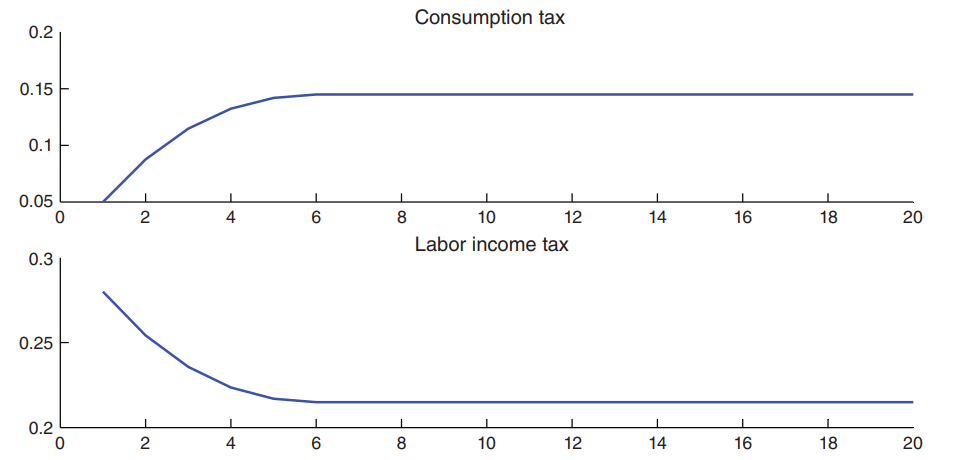
\includegraphics[width=0.7\linewidth]{images/correia2013}
	\caption{Dynamic Path for Unconventional Taxes, Sticky Prices, Flexible Wages}
	\small{Time, measured in quarters, is on the horizontal axis. Taxes are measured in levels}
	\label{fig:correia2013}
\end{figure}
\bb
Thus, \cite{correia2013unconventional} find that when facing a preference shock, there exists a path for both labor and consumption taxes that ensures a smooth transition back to the steady state. This approach carefully balances the adjustments in taxes to manage inflationary pressures without causing significant disruptions to the economy. The dynamic path illustrated in Figure \ref{fig:correia2013} demonstrates how these tax adjustments unfold over time, showing a gradual return to equilibrium.



\section{The Behavioural Model}
We now look to introduce behavioural aspects into what is currently a more traditional New Keynesian model consisting solely of perfectly rational agents. The ensuing Behavioural New Keynesian model has the same structure as the standard model. Inter-temporal household decisions are governed by an Euler-equation, while firms' pricing decisions are represented by a Phillips-curve, and monetary and fiscal policies are implemented via feedback rules. Yet, unlike the standard model, expectations are not fully rational. Instead, they are behavioural, reflecting the fact that agents do not have complete information and perceive more distant events as increasingly uncertain. This leads to higher cognitive discounting of forward-looking behavior and the inclusion of perception parameters within the structural relationships. These perception parameters alter the cross-equation and cross-coefficient restrictions that the standard model would imply, thereby influencing the dynamic behavior of the model variables in ways that can be significantly different from those predicted by the traditional framework. 

\subsection{General Approach}
Behavioural macroeconomics attempts to incorporate the idea that expectation formation is not necessarily based on perfect knowledge about the future evolution of all economically relevant variables \parencite{woodford2013macroeconomic}. Instead of possessing perfectly accurate forecasts, agents in this model may hold perceptions of reality that are imprecise and not entirely forward-looking. Under rational expectations, agents are assumed to have complete and perfect knowledge about the potential future paths of all variables. However, in practice, there are likely to be variables for which forming such precise expectations is challenging. This can be modelled as agents discounting the information that would otherwise be fully utilized by a rational agent. Various behavioural models incorporate this feature, including those with rationally inattentive agents, agents engaged in signal extraction, or those employing simple learning mechanisms. As a result, cognitive discounting leads to decision rules that, while appearing similar to those in standard rational expectations models, are adjusted to account for the behavioural deviations from full rationality.
\bb
In order to make a behavioural macroeconomic model internally consistent, two key elements are needed. First, an expectation formation mechanism that is consistent with the informational structure of the model economy, while boundedly rational. More specifically, the resulting deviations from fully rational expectations are not ad hoc but are subject to internal discipline and consistency. \cite{gabaix2014sparsity, gabaix2016behavioral} show how to derive an appropriate expectations operator via the concept of sparse dynamic programming. Second, a researcher still has to make assumptions on the agents' information set, or specifically, what economically relevant information the agents perceive. Looking at \cite{lubik2021fiscal}, we can see a concise summary of this from which I will expand on.

\bb
Consider a state variable $\boldsymbol{X}_t$ (comprising productivity $A_t$, preference shocks $\zeta_t$, as well as announced actions in monetary and fiscal policy), that will evolve in equilibrium as:
\begin{align}
	\boldsymbol{X}_{t+1} = \boldsymbol{G^X}(\boldsymbol{X}_t, \boldsymbol{\epsilon}_{t+1})
\end{align} 
for some equilibrium transition function $\boldsymbol{G^X}$ and mean-0 innovations $\boldsymbol{\epsilon}_{t+1}$ (which depend on the equilibrium policies of the agent and the government). If we assume that $\boldsymbol{X}_t$ has a mean 0 and linearise, we get:
\begin{align}
	\boldsymbol{X}_{t+1} = \boldsymbol{\Gamma X}_t + \boldsymbol{\epsilon}_{t+1}
\end{align}
where $\boldsymbol{\Gamma}$ is a matrix of coefficients and the vector $\boldsymbol{\epsilon}_{t+1}$ represents innovations to the dynamic system which are typically assumed to have zero mean and are \textit{i.i.d}. This equation therefore captures all the information that is potentially available to the agent. 
\bb
In our behavioural environment however, we assume that agents can be cognitively limited and thus perceive a modified version of the equation in which they do not fully perceive future changes in state variables. Hence we modify the equation to account for this:
\begin{align}
	\boldsymbol{X}_{t+1} = M\boldsymbol{G^X}(\boldsymbol{X}_t, \boldsymbol{\epsilon}_{t+1}) = M(\boldsymbol{\Gamma X}_t + \boldsymbol{\epsilon}_{t+1})
\end{align}
where M is a matrix containing corresponding cognitive discounting parameters. Each of these parameters take a value between 0 and 1. In the case the rational agent, they perfectly perceive the future path of each state variable, hence they are characterised by a parameter value of 1. Behavioural agents on the other hand, do not and so are characterised by parameter values below 1. 
Under expectation, the innovations disappear. The expectation of a cognitively limited agent is thus $ \mathbb{E}_t^{BR} \boldsymbol{X}_{t+1} = M\boldsymbol{\Gamma X}_t $ while that of the rational agent is simply:  $\mathbb{E}_t \boldsymbol{X}_{t+1} = \boldsymbol{\Gamma X}_t $. Therefore:
\begin{align}
	\label{eq:lemma}
	 \mathbb{E}_t^{BR} \boldsymbol{X}_{t+1} = M \:\mathbb{E}_t \boldsymbol{X}_{t+1}
\end{align}
Iterating over time, we can see that:
\begin{align}
	\mathbb{E}_t^{BR} \boldsymbol{X}_{t+k} = M^k \:\mathbb{E}_t \boldsymbol{X}_{t+k}
\end{align}
Recalling that each of the parameters within $M$ are contained between 0 and 1, we see that the more distant the events in the future, the more the behavioural agent ``sees them dimly", i.e. sees them with a dampened cognitive discount factor $M^k$ at horizon $k$. In light of this, behavioural macroeconomics results in the idea of a ``discounted Euler-equation.''

\subsection{The Behavioural Euler Equation}
In a standard New Keynesian framework, the Euler equation governs the time path of output by linking it to the real interest rate and aggregate shocks, reflecting the inter temporal consumption-savings choices made by households. The Behavioural Euler Equation shares the same foundational structure, but it incorporates a critical departure from the traditional model by assuming that agents do not fully observe or process all available information. Instead, they focus on a subset of key economic variables, leading to a more simplified and cognitively constrained decision-making process.
\bb
Building on the earlier discussion of cognitive discounting, where agents' expectations about future variables are attenuated by the matrix \( M \) (as shown in Equation \ref{eq:lemma}), this adjustment carries over to the Euler equation. In the behavioural framework, the agents' perception of future consumption, prices, and taxes is not perfectly aligned with the actual expected values. Instead, these perceptions are "discounted" according to the attention parameters, which reflect the degree of imperfect cognition.
\bb
This leads to a modified version of the Euler equation where the marginal utility of consumption today, denoted as \( u_C(C_t, N_t) \), is related to the expected discounted utility of future consumption, \( \mathbb{E}_t^{BR} u_C(C_{t+1}, N_{t+1}) \), adjusted for the nominal interest rate \( 1+i \), the ratio of preference shocks \( \frac{\xi_{t+1}}{\xi_t} \), the ratio of current to future prices \( \frac{P_t}{P_{t+1}} \), and the relative consumption tax adjustments \( \frac{(1+\tau_t^c)}{(1+\tau_{t+1}^c)} \). The Behavioural Euler Equation is expressed as:

\begin{align}
	\label{eq: intertemporal_BR}
		u_C(C_t, N_t) =& (1+i) \beta \mathbb{E}_t^{BR} u_C(C_{t+1}, N_{t+1}) \dfrac{\xi_{t+1}}{\xi_t}\dfrac{P_t}{P_{t+1}} \dfrac{(1+\tau_{t}^c)}{(1+\tau_{t+1}^c)}.
\end{align}
Using equation \ref{eq:lemma}, we can rewrite this as:
\begin{align}
	\label{eq:euler_br}
	u_C(C_t, N_t) =& (1+i) \beta M \mathbb{E}_t u_C(C_{t+1}, N_{t+1}) \dfrac{\xi_{t+1}}{\xi_t}\dfrac{P_t}{P_{t+1}} \dfrac{(1+\tau_{t}^c)}{(1+\tau_{t+1}^c)}.
\end{align}

Linearising this we get:
\begin{align}
	\tilde{C}_t = M\mathbb{E}_t \tilde{C}_{t+1}  - \dfrac{1}{\sigma}(i_t - \mathbb{E}_t \pi_{t+1} -r^{e}_t) + \dfrac{1}{\sigma}\mathbb{E}_t(\tilde{\tau}_{t+1}^c - \tilde{\tau}_{t}^c)
\end{align}
\textbf{As government spending is held constant we know that any deviation in income must be associated with a deviation in consumption, we can rewrite the previous equation:
}
\begin{align}
	\hat{y} = M\mathbb{E}_t \hat{y}_{t+1}  - \sigma(i_t - \mathbb{E}_t \pi_{t+1} - r_t^n) + \sigma(\mathbb{E}_t \hat{\tau}_{t+1}^c - \hat{\tau}_{t}^c )
\end{align}
where the natural rate of interest or discount rate is:
\begin{align}
	r_t = \big( \: ln\beta^{-1} - \bar{m} \mathbb{E}_t \hat{\xi}_{t+1} + \hat{\xi}_t \: \big) 
\end{align}


\subsection{The Behavioural Philips Curve}
The Phillips curve in a standard New Keynesian  model is fundamentally based on the concept of price stickiness, where firms do not adjust prices instantly in response to economic changes. This principle extends to the behavioural Phillips curve when cognitive discounting is introduced. In this context, we assume that decision-makers at firms do not fully account for the future state of the economy, reflecting limited attention or imperfect cognition. The derivation of the behavioural Phillips curve largely follows the traditional steps of the NK price-setting problem. As a result, we focus  only on the novel elements that arise from incorporating behavioural considerations.

\textbf{In this behavioral framework, each firm that produces a distinct variety 
??
i retains full control over its price-setting decisions. The optimal relative price 
??
??
,
??
+
??
P 
t,t+k
?}
is determined by maximizing the firm's profit, taking into account the imperfect attention to future economic conditions.


\begin{align}
	max\mathbb{E}_t^{BR} \sum_{k=0}^{\infty} (\theta \beta)^k \lambda_{t+k} \big[P_{t+k}Y_{t+k} - W_{t+j}Y_{t+k} \big] 
\end{align}



Following the usual steps for Calvo price-setting, we can then derive the behavioural Phillips curve:

\begin{align}
	\tilde{\pi}_t = \beta M^f \mathbb{E}_t \tilde{\pi}_{t+1} + \kappa \tilde{mc}_t,
\end{align}

where the coefficients are given by:

\begin{align}
	M^f &= m \left[ \theta + (1 - \theta)m_\pi \right]\\
	\kappa &= \frac{(1 - \theta\beta)(1 - \theta)}{\theta} m_x
\end{align}



\begin{align}
	\pi_t = \beta M^f \mathbb{E}_t \pi_{t+1} + \kappa \hat{y}_t + \kappa \psi(\hat{\tau}_{t}^n +\hat{\tau}_{t}^c) 
\end{align}

\subsection{Tax Implications}
As in \cite{eggertsson2011fiscal} and \cite{christiano2011government} we consider specific preferences as:
\begin{align}
	u(C_t, N_t, \xi_t) = u(C_t, N_t)\xi_t
\end{align}
In this way, the preference shock does not affect the marginal rate of substitution between consumption and leisure. It will, however, affect the marginal rate of substitution between consumption at time $t$ and consumption at time $t + 1$. We also assume, as in \cite{correia2013unconventional}, that $G_t = G$, $A_t = 1$, so that the only shock is the preference shock.


This results in an efficient allocation which is constant and unaffected by the preference shock:
\begin{align}
	- \dfrac{U_N(C_t,N_t)}{U_C(C_t,N_t)} = \dfrac{1}{A_t} = 1
\end{align}
and
\begin{align}
	C_t + G = A_tN_t = N_t
\end{align}
We modify the original 
\begin{align}
	\tilde{\xi}_t U'(C_t) = E_t^{BR}\left[\beta \tilde{\xi}_{t+1} U'(C_{t+1}) (1 + r_{t+1})\right]\\
	\tilde{\xi}_t U'(C_t) = \beta \bar{m} {\xi}_{t+1}E_t\left[ U'(C_{t+1}) (1 + r_{t+1})\right]
\end{align}


\bb
Therefore, in accordance with \cite{correia2013unconventional}, we set the perceived path of consumption taxes to: 
\begin{align}
	\dfrac{(1+\tau_{t+1}^c)}{(1+\tau_{t}^c)} = \beta \dfrac{\bar{m}\xi_{t+1}}{\xi_t}
\end{align}
and we set labour taxes equal to:
\begin{align}
	\dfrac{(1+\tau_{t}^c)}{(1-\tau_{t}^n)} \dfrac{\theta}{\theta-1} &= 1\\
	(1+\tau_{t}^c)\dfrac{\theta}{\theta-1} &= (1-\tau_{t}^n)
\end{align}



\subsection{Impact of a Negative Preference Shock on Our Results}
In line with \cite{correia2013unconventional}, we consider using a combination of consumption and labour taxes to mitigate the impact of such a shock. However, the presence of cognitive discounting changes the effectiveness of this strategy.
To counteract the decrease in consumption caused by the shock, the model would suggest lowering consumption taxes temporarily. This reduction would increase consumer prices, attempting to induce consumption by making future consumption relatively more expensive. However, under cognitive discounting, the impact of this tax reduction is amplified in the short term due to the heightened sensitivity of agents to current-period incentives. While this might initially boost consumption, the behavioural response could lead to excessive volatility, with agents overreacting to the temporary changes in taxes. To stabilize producer prices and prevent a decrease in marginal costs that could lead to deflation, a simultaneous increase in labour taxes would be necessary. However, as cognitive discounting causes agents to place more weight on immediate costs, the negative impact of higher labor taxes on labor supply would be more pronounced. This could deepen the recessionary effects by further reducing output and employment in the short term.
Over time, as the effects of the negative preference shock fade (i.e., as the shock becomes neutral after period \( T \)), consumption taxes would need to increase, and labour taxes decrease, to stabilize the economy. The key challenge in our model is managing the transition period, where the interplay between cognitive discounting and tax adjustments could lead to greater economic instability than in a standard rational expectations framework.
\bb
Post-shock, the model would prescribe an increase in consumption taxes to stabilize prices and restore the natural rate of interest to positive levels. However, the persistence of cognitive discounting means that agents might under-react to this increase, leading to prolonged periods of low consumption and delayed economic recovery. Similarly, reducing labour taxes would be necessary to encourage labor supply and increase output. But again, cognitive discounting might cause agents to undervalue the future benefits of lower taxes, resulting in a slower than expected response in labour market recovery.
\bb
In traditional models like those of \cite{eggertsson2011fiscal} and \cite{correia2013unconventional}, the response to a negative preference shock is more straightforward. Lowering consumption taxes and raising labour taxes can effectively manage the recessionary effects by inducing inflation and stabilizing producer prices. However, our model introduces additional complexity due to the behavioural biases of agents. The primary difference is the increased volatility in response to tax changes. While traditional models predict a smooth transition back to equilibrium, our model suggests that cognitive discounting leads to overreactions and under-reactions that complicate the policy response. The need for more careful calibration of tax policies is also highlighted. Small errors in timing or magnitude of tax adjustments could have outsized effects due to the exaggerated behavioural responses under cognitive discounting. Thus, a negative preference shock in our model exacerbates the challenges of using tax policy to stabilize the economy, particularly in the presence of cognitive discounting. While the basic principles of adjusting consumption and labour taxes still apply, the behavioural distortions introduced by cognitive discounting necessitate a more cautious and dynamic approach to policy implementation. The risk of increased economic volatility and prolonged recovery underscores the importance of understanding and accounting for behavioural factors in macroeconomic policy design.



\subsection{Time Consistency}
The introduction of cognitive discounting




\subsection{Sales Tax vs VAT}
It is important to note that the introduction of cognitive discounting in our model does not necessarily provide any further support for reducing value-added taxes (VAT). As emphasized by \cite{eggertsson2011fiscal}, VAT, which is commonly used in Europe, interacts with price frictions differently compared to American sales taxes. In the case of sales taxes, our model assumes that firms set prices based solely on the tax, so a 1\% reduction in the tax directly translates into a 1\% lower purchasing price for consumers, even if firms do not immediately adjust their prices.
\bb
However,\cite{eggertsson2011fiscal} argues that this assumption is less plausible for VAT, where prices are typically inclusive of the tax due to legal requirements. In his analysis, if firms post prices that include VAT, a 1\% reduction in VAT will only be reflected in consumer prices if firms adjust their pricing decisions, which occurs at stochastic intervals in the model. Therefore, as highlighted in \cite{eggertsson2004optimal} , VAT affects the aggregate supply (AS) and aggregate demand (AD) equations in a manner similar to payroll taxes, leading to an unchanged analysis in our framework.
\bb
This implies that while sales tax cuts can be expansionary due to an immediate decrease in consumer prices and expected higher future prices, VAT cuts might have the opposite effect. Because VAT is included in posted prices, a reduction in VAT will only be apparent once firms revise their prices, which could delay the observed impact and lead consumers to postpone purchases in anticipation of future lower prices. Consequently, reducing VAT might be contractionary, as firms' delayed price adjustments affect consumption behaviour.





\textbf{
As in behavioural forces don't change the natural rate of output directly here, but they do change the pure natural rate of interest.}






\section{Introducing Deficit financing}
\cite{gabaix2020behavioural} outlines how the addition of behavioural agents generates a failure of Ricardian equivalence. In traditional New Keynesian models with rational, forward-looking agents, such as those analysed in \cite{eggertsson2011fiscal}, Ricardian equivalence suggests that the method of government financing, whether through lump-sum taxes or debt issuance, should have no impact on overall economic activity. Under this theory, rational agents anticipate future tax liabilities that will arise from government debt and, therefore, adjust their savings accordingly, neutralizing the impact of debt-financed government spending on consumption and output.
\bb
However, when behavioural agents are introduced into the model, this equivalence breaks down. Behavioural agents, characterized by bounded rationality, cognitive biases, or myopia, do not fully account for the future tax implications of government debt. As a result, they may perceive government borrowing as an increase in their net wealth, leading to higher current consumption and a corresponding boost in aggregate demand. This divergence from traditional rational behaviour creates room for government debt to influence the real economy in ways that are not predicted by classical models. The failure of Ricardian equivalence in the presence of behavioural agents suggests that deficit financing could have significant short-term effects on consumption and output, a possibility that warrants further exploration within the context of macroeconomic models that incorporate these behavioural considerations.
\bb
In our previous analysis, we maintained a fixed level of government spending and attributed variations in tax rates solely to preference shocks. This approach allowed us to examine the immediate effects of these shocks without delving into the complexities of fiscal policy adjustments. However, this framework simplifies the reality where governments often need to adjust spending and taxes dynamically to respond to economic conditions. In more realistic scenarios, governments face liquidity constraints that can limit their ability to raise taxes sufficiently to cover desired levels of spending, particularly during economic downturns. Consequently, governments frequently resort to deficit financing, issuing debt to bridge the gap between expenditures and revenues. To further explore the effects of these deficits on our model we incorporate deficit dynamics. This adjustment enables us to investigate the impact of increased government debt on the output gap in the case of behavioural agents.
\bb
To do this we adopt the approach outlined by \cite{uhlig2010some}, where the debt dynamics post-spending shock are characterized by the following equation:
\begin{align}
	B_{t+1} - \bar{B} = (1-\psi)(d_t - \bar{d}), \qquad\qquad \psi \in [0,1]
\end{align}
where;
\begin{align*}
	d_t = \dfrac{r}{R}B_t + g_t - T_t - \tau^c c_t
\end{align*} 
The cost of servicing existing debt is represented by \( \dfrac{r}{R}B_t \), while \( g_t \) is government spending, \( T_t \) denotes tax revenues from lump-sum taxes, and \( \tau^c c_t \) reflects the revenue from consumption taxes. Furthermore, \( B_{t+1} \) is the debt level at time \( t+1 \), and \( \bar{B} \) represents the steady-state debt level. Similarly, \( d_t \) is the deficit at time \( t \), and \( \bar{d} \) is its steady-state counterpart. The parameter \( (1-\psi) \) indicates the fraction of the deficit that is financed through debt issuance. When \( \psi = 1 \), all additional spending is financed through taxes, while when \( \psi = 0.1 \), 10\% of the additional spending is covered by tax increases, and the remaining 90\% is financed through increased debt.
\bb
Notice that in this version of our model, in accordance with \cite{uhlig2010some}, taxes on consumption remain constant over time and labour taxes adjust to solve the model. This is in stark contrast with the method outlined in \cite{correia2013unconventional} analysed above. 
\bb
Unlike traditional New Keynesian models with perfectly rational agents, debt dynamics in our behavioural model will therefore have 

 

\subsection{An Approximated Equilibrium}
\begin{align}
	\hat{y} = M\mathbb{E}_t \hat{y}_{t+1} + b_d (1-\psi)\hat{d}_t  - \sigma(i_t - \mathbb{E}_t \pi_{t+1} - r_t^n)  + b_g\left(M\mathbb{E}_t \hat{g}_{t+1} - \hat{g}_t\right)
\end{align}
Where the sensitivity of the output gap to deficits is;
\begin{align*}
	b_d = \dfrac{\phi r  R (1- \bar{m})}{(\phi + \sigma) (R-\bar{m})} 
\end{align*}
In the case of rational, forward-looking agents $M = \bar{m} = 1$, resulting in $b_d = 0$. This gives us the traditional case in which the output gap is not sensitive to deficits, reflecting the traditional Ricardian equivalence principle. However, in the case of behavioural agents, where $0 \leq \bar{m} < 1$, agents do not fully internalize the future tax burden of deficit-financed spending and so view it as an increase in net-wealth. They subsequently adjust their spending accordingly, reducing the output gap relative to the steady state. This breaks from  the traditional Ricardian equivalence and highlights the significant impact deficits can have on economic activity when agents deviate from rational expectations.
\bb
Superficially, the deficit portion of this IS equation looks very similar to equation 162 found in the online appendix of \cite{gabaix2020behavioural} however, the dynamics are very different. 
\bb
Notice that in this version of the model, $\sigma(M\mathbb{E}_t \hat{\tau}_{t+1}^c - \hat{\tau}_{t}^c )$ disappears as taxes on consumption are now constant over time. Yet, because we have loosened the restrictions on government spending, we now include $b_g\left(M\mathbb{E}_t \hat{g}_t - \hat{g}_t\right)$, which captures the dynamic impact of government spending changes on the output gap. 
\bb
The Phillips curve in this model retains its traditional form but is now influenced by the changes in government spending, which have been integrated into the output gap dynamics. While deficits themselves do not directly affect the Phillips curve, the relaxed restrictions on government spending introduce a significant channel through which fiscal policy can influence inflationary pressures. Specifically, deviations of government spending from its steady-state level are now explicitly incorporated into the Phillips curve equation.
\begin{align}
	\pi_t &= \beta M \mathbb{E}_t \pi_{t+1}  + \kappa \hat{y}_t  +\kappa \psi (\tilde{\tau}_t^c + \tilde{\tau}_t^n + \hat{g_t})
\end{align}


\subsection{Fiscal Multiplier}





\section{Conclusion}
This paper has sought to expanded upon work done by \cite{gabaix2020behavioural} and his Behavioural New Keynesian framework by incorporating distortionary taxes, thereby enhancing our understanding of fiscal policy in an environment where agents exhibit cognitive biases. By integrating cognitive discounting into the analysis of labour and consumption taxes, we have demonstrated that traditional macroeconomic results, which assume rational expectations, may not fully capture the complexities introduced by behavioural factors. Specifically, we have shown that cognitive discounting can significantly alter the standard trade-offs associated with distortionary taxes, notably the volatility shown in  decisions in ways that differ markedly from those predicted by models relying solely on rational expectations.
\bb
Moreover, our exploration of deficit financing within this behavioural framework has yielded important insights into the dynamics of debt and fiscal sustainability under bounded rationality. We found that the interaction between cognitive discounting and deficit financing can affect economic multipliers and long-term outcomes, challenging the conventional wisdom derived from rational expectation models. These findings underscore the importance of accounting for cognitive biases when designing and implementing fiscal policies, particularly in situations involving significant government spending and debt accumulation.
\bb
Our analysis provides a foundation for future research into the broader implications of cognitive discounting in macroeconomic modelling. The results presented here suggest several avenues for further exploration, such as the inclusion of distortionary taxes in heterogeneous agent models,  such as the one developed by \cite{pfauti2022behavioral}, and the investigation of progressive taxation, such as \cite{ferriere2024heterogeneous}, within a behavioural context. By extending our framework to incorporate these complexities, future work could yield even deeper insights into the distributional effects of fiscal policy and the role of behavioural biases in shaping economic outcomes.
\bb
In conclusion, this paper contributes to the growing literature on Behavioural New Keynesian economics by offering a more nuanced perspective on fiscal policy in the presence of cognitive limitations. Our findings highlight the need for policymakers to consider the potential distortions introduced by behavioural biases, particularly in the design and implementation of tax policies and deficit-financed spending programs. As governments continue to navigate complex economic environments, the integration of behavioural insights into macroeconomic models will be crucial for developing more effective and realistic policy interventions.



	



\pagebreak
\printbibliography


\pagebreak
\section{Appendix: The log-linearized model}
Naturally, our log-linearised process is very similar to that found in \cite{correia2013unconventional}.

\subsection{Behavioural Euler Equation}
If we log-linearize equation \ref{eq: intertemporal_BR}, we obtain:
\begin{equation}
	\delta \hat{C}_t + \Gamma \hat{\xi}_t - \hat{\tau}^c_t =  \left[\hat{i}_t - \ln\left(\frac{1}{\beta}\right) - \mathbb{E}_t \pi_{t+1}\right] + \mathbb{E}_t^{BR} \left[\delta \hat{C}_{t+1} + \Gamma\hat{\xi}_{t+1} - \hat{\tau}^c_{t+1}\right]
\end{equation}
where $\delta = \dfrac{C }{u_c}(u_{CC }+ u_{CN })$, and $\hat{C}_t = \ln\left(\frac{C_t}{C}\right)$,  $\hat{\tau}^c_t = \ln\left(\frac{1+\tau^c_t}{1+\tau^c}\right)$, and $\pi_{t+1} = \ln\left(\frac{P_{t+1}}{P_t}\right)$.  Notice, that  the expectation term in front of inflation $\mathbb{E}_t \pi_{t+1}$, in the IS curve remains unaffected and does not incorporate any behavioural biases. This is because our model does not contain the concept of nominal illusion. One could include it as outlined in a footnote by \cite{gabaix2020behavioural}, yet for   we do not. 
Furthermore,  we know that because $\xi$ is multiplicative, deviations between periods effects consumption proportionally, hence we can say $\Gamma = 1$ and rewrite the equation as follows;

\begin{equation}
	\delta \hat{C}_t +  \hat{\xi}_t - \hat{\tau}^c_t =  \left[\hat{i}_t - \ln\left(\frac{1}{\beta}\right) - \mathbb{E}_t \pi_{t+1}\right] + \mathbb{E}_t^{BR} \left[\delta \hat{C}_{t+1} + \hat{\xi}_{t+1} - \hat{\tau}^c_{t+1}\right]
\end{equation}
assuming that government consumption is constant, delivers


\begin{align*}
	\frac{C}{C + G} \hat{C}_t = \hat{y}_t
\end{align*}
So, if we let  $g^{-1} = \frac{C}{C + G}$,  then
\begin{align*}
	\hat{C}_t = g\hat{y}_t,
\end{align*}
Then we can rewrite the equation as:
\begin{equation}
	\delta g\hat{y}_t +  \hat{\xi}_t - \hat{\tau}^c_t =  \left[\hat{i}_t - \ln\left(\frac{1}{\beta}\right) - \mathbb{E}_t \pi_{t+1}\right] + \mathbb{E}_t^{BR} \left[\delta g\hat{y}_{t+1} + \hat{\xi}_{t+1} - \hat{\tau}^c_{t+1}\right]
\end{equation}
Hence, using \ref{eq:lemma}, we are left with: 
\begin{equation}
	\delta g\hat{y}_t +  \hat{\xi}_t - \hat{\tau}^c_t =  \left[\hat{i}_t - \ln\left(\frac{1}{\beta}\right) - \mathbb{E}_t \pi_{t+1}\right] + M \mathbb{E}_t \left[\delta g\hat{y}_{t+1} + \hat{\xi}_{t+1} - \hat{\tau}^c_{t+1}\right]
\end{equation}
Ultimately we can write the IS equation as:
\begin{equation}
	\hat{y}_t \approx M \mathbb{E}_t \hat{y}_{t+1} + \sigma \left[\hat{i}_t - \mathbb{E}_t \pi_{t+1} - \left(\ln\beta^{-1} + \hat{\xi}_t - M \mathbb{E}_t \hat{\xi}_{t+1}\right)\right] - \sigma \left[M \mathbb{E}_t \hat{\tau}^c_{t+1} - \hat{\tau}^c_t\right]
\end{equation}

\subsection{Behavioural Philips Curve}
As productivity shocks play no particular role, we assume that $A_t = 1$ for all $t$, such that:

\begin{equation}
	\frac{p_t}{P_t} = \left(\frac{\epsilon-1}{\epsilon}\right) \mathbb{E}_t^{BR} \left[\sum_{j=0}^{\infty} (1-\beta \theta)(\beta \theta)^j \frac{W_{t+j}}{P_{t+j}}\right]
\end{equation}
The steady state has $C_t = C$, $N_t = N$, $\xi_t = 1$, $\tau^c_t = \tau^c$, $\tau^n_t = \tau^n$, $P_t = p_t = P$, and $1+i = \beta^{-1}$, so that $\frac{\epsilon-1}{\epsilon} W = P$.
\bb
Linearising this we get;
\begin{align*}
	\ln p_t &\simeq \ln \left(\frac{\theta}{\theta - 1}\right) + \ln \mathbb{E}_t^{BR} \sum_{j=0}^{\infty} (1-\beta \theta)(\beta \theta)^j W_{t+j} 
\end{align*}
Where $W_t$ is;
\begin{align*}
			W_t &= \frac{\left(1 + \tau^c_t\right) P_t}{\left(1 - \tau^n_t\right)} 
		\left[\frac{u_C\left(C_t, N_t\right)\xi_t}{u_N\left(C_t, N_t \right)\xi_t}\right]^{-1} 
\end{align*}
Notice that as $\xi$ is multiplicative, $\dfrac{\xi_t}{\xi_t}$ cancels out and so has no impact on the Philips curve.
\begin{align*}
	\ln p_t &\simeq \ln \left(\frac{\theta}{\theta - 1}\right) + \ln \mathbb{E}_t^{BR} \sum_{j=0}^{\infty} (1-\beta \theta)(\beta \theta)^j
	\left(\frac{\left(1 + \tau^c_{t+j}\right) P_{t+j}}{\left(1 - \tau^n_{t+j}\right)}\right) 
	\left[\frac{u_C\left(C_{t+j}, N_{t+j}\right)}{u_N\left(C_{t+j}, N_{t+j}\right)}\right]^{-1} \\
	\ln p_t - \ln P_t &\simeq \ln \left(\frac{\theta}{\theta - 1}\right) + \ln \mathbb{E}_t^{BR} \sum_{j=0}^{\infty} (1-\beta \theta)(\beta \theta)^j
	\left(\frac{\left(1 + \tau^c_{t+j}\right) \frac{P_{t+j}}{P_t}}{\left(1 - \tau^n_{t+j}\right)}\right) 
	\left[\frac{u_C\left(C_{t+j}, N_{t+j}\right)}{u_N\left(C_{t+j}, N_{t+j}\right)}\right]^{-1}
\end{align*}

The log-linearization of the second term on the right-hand side is given by
\begin{align*}
	\ln \mathbb{E}_t^{BR} \sum_{j=0}^{\infty} (1-\beta \theta)(\beta \theta)^j
	&\left(\frac{\left(1 + \tau^c_{t+j}\right) \frac{P_{t+j}}{P_t}}{\left(1 - \tau^n_{t+j}\right)}\right) 
	\left[\frac{u_C\left(C_{t+j}, N_{t+j}\right)}{u_N\left(C_{t+j}, N_{t+j}\right)} \right]^{-1} 
	\simeq (1 - \alpha \beta) \mathbb{E}_t^{BR} \sum_{j=0}^{\infty} (\alpha \beta)^j [\Omega_{t+j}]
\end{align*}
where
\begin{align*}
	\Omega_{t+j} = \hat{\tau}^c_{t+j} + \hat{\tau}^n_{t+j} + \pi_{t+j} + \phi \hat{C}_{t+j} 
\end{align*}
where; 
\begin{align*}
	\pi_t(j) = \ln \frac{P_{t+j}}{P_t} \\
	\hat{\tau}^n_t = \frac{\left(1 - \tau^n_t\right)}{\left(1 - \tau^n\right)}
\end{align*}
Then we can write:
\begin{align*}
	\pi_t \simeq (1 - \alpha \beta) \frac{1 - \alpha}{\alpha} 
	\left[\tilde{\tau}_t^c + \tilde{\tau}_t^n + \phi \hat{C}_t - \gamma \hat{\xi}_t \right] 
	+ \frac{1 - \alpha}{\alpha} (\alpha \beta) \mathbb{E}_t^{BR} [\pi_{t+1}] 
	+ (\alpha \beta) \mathbb{E}_t^{BR} \pi_{t+1}
\end{align*}
or
\begin{align*}
	\pi_t = (1-\theta \beta) \dfrac{1-\theta}{\theta} \left[\hat{\tau}^c_{t+j} + \hat{\tau}^n_{t+j} +  \phi \hat{C}_{t+j}\right] + \beta \mathbb{E}_t^{BR} \pi_{t+1}
\end{align*}
Using \ref{eq:lemma} we transform this into; 
\begin{align*}
	\pi_t = (1-\theta \beta) \dfrac{1-\theta}{\theta} \left[\hat{\tau}^c_{t+j} + \hat{\tau}^n_{t+j} +  \phi \hat{C}_{t+j}\right] + \beta M \mathbb{E}_t \pi_{t+1}
\end{align*}
\bb
Finally, remember that;
\begin{align*}
	\hat{C}_t = g \hat{y}_t, 
\end{align*}
Therefore: 
\begin{align*}
	\pi_t \simeq (1 - \alpha \beta) \frac{1 - \alpha}{\alpha} 
	\left[\tilde{\tau}_t^c + \tilde{\tau}_t^n + \phi g \hat{y}_t \right] 
	+ \beta M \mathbb{E}_t \pi_{t+1},
\end{align*}
Setting; 
\begin{align*}
	M &= \bar{m}\\
	\kappa &= (1 - \alpha \beta) \frac{1 - \alpha}{\alpha} \phi g, \\
	\psi &= (\phi g)^{-1},
\end{align*}
This leaves us with a behavioural Phillips curve: 
\begin{align*}
	\pi_t &\simeq \beta M \mathbb{E}_t \pi_{t+1}  + \kappa \hat{y}_t  +\kappa \psi (\tilde{\tau}_t^c + \tilde{\tau}_t^n)
\end{align*}



\end{spacing}
\end{document}



